\title{International Attitudes Toward Global Policies %
} 

\begin{abstract}
  %

  We document majority support for policies entailing global redistribution and climate mitigation. Surveys on 40,680 respondents in 20 countries show strong stated support for an effective way to jointly combat climate change and poverty: a global carbon price funding a global basic income, called the ``Global Climate Scheme'' (GCS). Using complementary surveys on 8,000 respondents in the U.S., France, Germany, Spain, and the UK, we test several hypotheses that could reconcile strong stated support with a lack of salience in policy circles. 
  The GCS is supported by three quarters of Europeans and half of Americans, even as they understand the policy's cost to them. Using different experiments, we show that the support for the GCS is sincere and that electoral candidates could win votes by endorsing it. More generally, we document widespread support for other globally redistributive policies, such as a wealth tax funding low-income countries or increased foreign aid. In sum, we provide evidence that global policies are genuinely supported by majorities, even in wealthy nations that would bear the burden.
  %
\end{abstract}

\textbf{JEL codes:} P48, Q58, H23, Q54 %

\textbf{Keywords:} Climate change, global policies, cap-and-trade, attitudes, survey.%

\tableofcontents

\onehalfspacing %
\section{Introduction}%
Major sustainability objectives could be achieved by global approaches to mitigating climate change and poverty involving transfers from high- to lower-income countries \citep{budolfson_climate_2021,franks_mobilizing_2018,dennig_inequality_2015,soergel_combining_2021,bauer_quantification_2020,cramton_global_2017}. For instance, a global wealth tax could finance the Sustainable Development Goals \citep{piketty_brief_2022}. More specifically, if merely 35\% of the revenue were allocated for this purpose, a global 2\% tax on individual wealth in excess of \$5 million could significantly reduce poverty as it would mechanically increase low-income countries' national income by 50\% (as computed on the \href{https://wid.world/world-wealth-tax-simulator/}{WID wealth tax simulator}). Besides, global carbon pricing is widely regarded by economists as the benchmark climate policy, as it would efficiently correct the carbon emissions externality. In an early analysis of global climate policy, \citet{grubb_greenhouse_1990} states: ``by far the best combination of long term effectiveness, feasibility, equity, and simplicity, is obtained from a system based upon tradable permits for carbon emissions which are allocated on an adult per capita basis'', i.e., equally among human adults. Support for such solution, which we call the ``Global Climate Scheme'', has been renewed ever since \citep{hoel_carbon_1991,agarwal_global_1991,bertram_tradeable_1992,baer_equity_2000,jamieson_climate_2001,blanchard_major_2021,rajan_global_2021}. 

While international negotiations have not yet led to ambitious globally redistributive policies, recent developments suggest that such a change might be underway. The International Maritime Organization is poised to adopt a global carbon levy on maritime fuel; the \citet{african_union_african_2023} calls for a global carbon taxation regime; the \citet{un_promotion_2023} is setting up a Framework Convention on International Tax Cooperation; Brazil uses its presidency of the G20 in 2024 to propose a global wealth tax, %
\href{https://www.lemonde.fr/idees/article/2023/03/14/taxation-mondiale-sur-les-ultrariches-ce-que-nous-avons-reussi-pour-les-multinationales-nous-devons-le-faire-pour-les-grandes-fortunes_6165354_3232.html}{backed} by 130 Members of the European Parliament; etc. 

A key condition for implementing global policies has remained largely unaddressed: the support of citizens. Using a Global survey on 40,680 respondents from 20 high- and middle-income countries, we reveal substantial support for those policies, especially global climate policies and a global tax on the wealthiest aimed at financing low-income countries (other questions from these surveys are analyzed in a companion paper, \citealp{dechezlepretre_fighting_2022}). Interestingly, even in wealthy nations that would bear a significant burden, majorities of citizens express support for such globally redistributive policies. To better understand public support for global policies in high-income countries, we conduct Complementary surveys among 8,000 respondents from France, Germany, Spain, the U.S., and the UK. 

By studying in depth the support for global policies, we are making an ambitious shift in the methodological approach of attitudinal surveys. In general, academic surveys focus on studying effect sizes of some treatment on political attitudes, or the socio-demographic factors that correlate with attitudes (e.g., \citealp{kuziemko_how_2015,douenne_yellow_2022}). The magnitude of support for a given proposal is often regarded as problematic to estimate satisfactorily. %
The measure of support is usually left to non-academic pollsters, who rarely apply all the academic best practices: transparency, representative sampling, neutral and precise wording of questions, comparison with existing literature, use of multiple questions and complementary methods to correctly interpret the results. Although it is challenging to estimate the extent of support, this question seems too important not to be addressed using scientific methods. Absent large scale measurements of public opinion like referenda, surveys remain the best method to assess support or opposition to given policies. In this paper, after a worldwide assessment in the Global survey, we use Complementary surveys to carefully measure the support for global policies in Western countries. We inquire the support for various policies, approach the question from diverse angles, and run a battery of pre-registered tests to check whether stated support estimates are reliable.

The focus of the Complementary surveys is a specific policy aimed at addressing both climate change and poverty, referred to as the ``Global Climate Scheme'' (GCS). It implements a cap on carbon emissions to limit global warming below 2\textdegree{}C. The emission rights are auctioned each year to polluting firms and fund a global basic income, alleviating extreme poverty. 
This archetypal policy exposes respondents to the key trade-off between the benefits and costs of globally redistributive climate policies, as respondents are made aware of the cost that the GCS entails for their country's people. 

After checking that respondents have understood the policy and its cost, we measure the support in a direct \textit{Yes}/\textit{No} question. The GCS is supported by three quarters of Europeans and more than half of Americans. Then, we test for social desirability bias using a list experiment. We find no evidence that people exaggerate their support in the direct question. To assess whether the support would diminish in a context with real stakes, we ask respondents whether they are willing to sign a petition in favor of the GCS, after informing them that the question results will be communicated to their head of state's office. The support is sustained in an environment that approaches real stakes. We then carry out conjoint analyses to neutralize experimenter demand and investigate the priority given to global policies compared to other types of policies. Conjoint analyses reveal that a political platform is more likely to be preferred if it contains the GCS or a global tax on millionaires, and that global policies rank high in the prioritization of policies. Our randomized experiments also show that a candidate would not lose vote intentions by endorsing the GCS, and might even gain up to 11 points in a country like France. An analysis of open-ended fields confirms that support for the GCS is real, and indicates that appeal of the GCS comes from its international nature and its impacts on climate, more than on global poverty. %
We also test other global policies and universalistic attitudes. Support is very strong for a global tax on millionaires, and the median respondent prefers to allocate 30\% of the revenues of such a tax to low-income countries. Majorities are willing to increase foreign aid, but only if some conditions are respected, such as making sure the aid is well spent and other high-income countries also increase their contribution. Questions on universalistic values, including a donation experiment, confirm the congruence of underlying values with the support for specific policies. Our diverse approaches also help understand what drives the support. For instance, the evidence indicates that one key reason why increasing foreign aid is not as popular as global policies lies in its unilateral nature. We reckon that survey evidence is no panacea, as attitudes can be ambivalent and context-dependent. Nevertheless, we arguably employ the best available methods to address potential concerns, including an experiment assessing how support might be affected by a negative media campaign. 

Overall, our results %
point out to strong and genuine support for global climate and redistributive policies, as our experiments confirm the stated support found in direct questions. This suggests that carefully administered surveys can be used to measure the level of support for a given policy. Our results contribute to the literature on attitudes toward climate policy, confirming that climate policy is preferred at a global level \citep{issp_international_2010,beiser-mcgrath_could_2019,sivonen_attitudes_2022,meilland_international_2023}, where it is more effective and fair. Indeed, the Global Climate Scheme is largely supported, but a similar policy at the national level is opposed by a majority in many countries \citep{dechezlepretre_fighting_2022}, despite lower costs. Noting that only 13\% of French people declared supporting a national carbon tax with cash transfers during the Yellow Vests movement \citep{douenne_yellow_2022}, surveys appear to accurately reflect the level of support. Therefore, unless support for global policies disappear once they enter the public debate, it seems unlikely that a policy such as the GCS would face major protests. 
In our discussion we offer potential explanations behind the lack of prominence of global policies in the public debate despite this strong support. 
Finally, while our findings underscore majority support for global policies, converging results from independent surveys are needed to ascertain such novel evidence. %
\paragraph{Literature} 

International surveys have shown widespread support for costly climate action \citep{dechezlepretre_fighting_2022,leiserowitz_international_2022}. For instance, using representative samples in 125 countries covering 96\% of the world's greenhouse gas emissions, \citet{andre_globally_2024} show that 69\% of the global population express willingness to contribute 1\% of their income to fight global warming. International surveys have also uncover near consensus that ``present economic differences between rich and poor countries are too large'' (overall, 78\% agree and 5\% disagree) in each of 29 countries \citep{issp_international_2019}. 

Yet, few prior attitudinal surveys have examined global redistributive policies. 
A notable exception is \citet{carattini_how_2019}, who test the support for six variants of a global carbon tax on samples in five countries, representative along gender and age. For a given variant, the sample size is about 167 respondents per country. They find over 80\% support for any variant in India, between 50\% and 65\% in Australia, the UK and South Africa, and 43\% to 59\% in the U.S., depending on the variant. Notably, the support for a global carbon tax funding an equal cash transfer for each human is close to 50\% in high-income countries (e.g., at 44\% in the U.S.). These figures are consistent with our results from the \textit{Global} survey (see Figure \ref{fig:oecd}), where the support is lower for a tax that would ``only'' reduce CO$_\text{2}$ emissions than for a quota that would unambiguously achieve the climate target. 
Relatedly, \cite{leiserowitz_public_2021} reveal that 66\% of Americans support providing ``financial aid and technical support to developing countries that agree to limit their greenhouse gas emissions''; and \citet{fehr_your_2022} find that 90\% of Germans want some degree of global redistribution. 
Besides, in surveys conducted in Brazil, Germany, Japan, the UK and the U.S., \citet{ghassim_who_2020} finds support ranging from 55\% to 74\% for ``a global democracy including both a global government and a global parliament, directly elected by the world population, to recommend and implement policies on global issues''. %
Through an experiment, he also finds that, in countries where the government stems from a coalition, voting shares would shift by 8 (Brazil) to 12 p.p. (Germany) from parties who are said to oppose global democracy to parties that supposedly support it. For instance, when Germans respondents were told that (only) the Greens and the Left support global democracy, these parties gained respectively 9 and 3 p.p. in vote intentions, while the SPD and the CDU-CSU each lost 6 p.p. 

Appendix \ref{sec:literature} contains a broader literature review including further attitudinal surveys on global policies (\ref{subsubsec:literature_attitudes_policies}); prior work on attitudes toward climate burden sharing (Appendix \ref{subsubsec:literature_attitudes_burden_sharing}), attitudes toward foreign aid (Appendix \ref{subsubsec:literature_foreign_aid}); global carbon pricing (Appendix \ref{subsubsec:literature_pricing}), global redistribution (Appendix \ref{subsubsec:literature_redistribution}), basic income (Appendix \ref{subsubsec:literature_basic_income}), and global democracy (Appendix \ref{subsubsec:literature_democracy}).

\section{Results}
The presentation of results proceeds as follows: after briefly describing the survey data (\ref{subsec:data}), we first document broad international support for global approaches to climate policy that lead to global redistribution (\ref{subsubsec:global_support}). Subsequently, we present specific findings from surveys in the U.S. and Europe that document support for the GCS, wealth taxes, and foreign aid in those countries (\ref{subsubsec:support_gcs}-\ref{subsubsec:support_foreign_aid}). We proceed to study the support for the Global Climate Scheme in more detail, by means of a list experiment, petition, conjoint analyses, prioritization task, and by eliciting pros and cons (\ref{subsec:robustness_sincerity}). To understand the gap between support for global policies and their appearance in public discussion, we conclude by reporting results on underlying universalistic values (\ref{subsec:universalistic}) and beliefs about the support of others (\ref{subsec:second_order_beliefs}). 

\subsection{Data}\label{subsec:data}

The study relies on two sets of surveys: the \textit{Global} survey and the \textit{Complementary} surveys (see Table \ref{tab:survey_summary}).
\renewcommand{\thetable}{S\arabic{table}}
\begin{table}[h]
  \caption[Surveys summary]{[For Supplementary Material] Summary of the surveys used in the analysis.}
  %
  \label{tab:survey_summary}
  \centering
\begin{tabular}
  {@{\extracolsep{5pt}}lcccc} 
  \\[-1.8ex]\hline 
  \hline \\[-1.8ex] 
   & \textit{Global survey} & \multicolumn{3}{c}{\textit{Complementary surveys}} \\
  \\[-1.8ex] Survey & \textit{Global} & \textit{Eu} & \textit{US1} & \textit{US2} \\ 
  \hline \\[-1.8ex]   
  Country coverage & 20 countries & FR, DE, ES, UK & U.S. & U.S. \\ 
  Sample size & 40,680 & 3,000 & 3,000 & 2,000 \\ 
  Main purpose & \makecell{Stated support \\for global policies} & \multicolumn{3}{c}{\makecell{Focus on GCS (sincerity, rationales, etc.) \\+ Support for global redistribution \\+ Universalistic values}} \\
  %
  %
  \hline 
  \hline \\[-1.8ex] 
\end{tabular}
\end{table}
\setcounter{table}{0}
\renewcommand{\thetable}{\arabic{table}}

\paragraph{Global Survey}

The \textit{Global} survey, conducted in 2021, involved 40,680 respondents from 20 countries, representing approximately 72\% of global CO$_\text{2}$ emissions. This survey serves as the basis for measuring stated support for various global policies worldwide. Detailed information about the data collection process, sample representativeness, and analysis of questions on national policies can be found in \citet{dechezlepretre_fighting_2022}.

\paragraph{Complementary Surveys}\label{par:surveys}

To delve deeper into the sincerity and rationales behind support for the GCS and attitudes towards global policies, global redistribution, and universalistic values, complementary surveys were conducted in 2023. These surveys are based on a sample of 8,000 respondents from France, Germany, Spain, the UK, and the U.S. The European survey (\textit{Eu}) comprises 3,000 respondents, while the U.S. sample was collected in two separate waves: \textit{US1} with 3,000 respondents and \textit{US2} with 2,000 respondents. The survey questions in both the European and U.S. surveys are identical, except for an additional question in \textit{US2} that uses results from \textit{US1} to assess the bandwagon effect.

The complementary surveys ensured representativeness along key dimensions: gender, income, age, highest diploma, and degree of urbanization. The \textit{Eu} survey is also representative of its four countries in terms of population size, while the \textit{US1} and \textit{US2} surveys are representative in terms of region and ethnicity. Tables \ref{tab:representativeness_waves}-\ref{tab:representativeness_EU} confirm that our samples closely match population frequencies. More detail on data collection is given in Section \nameref{sec:methods}. The questionnaires used in the surveys are provided in Appendices \ref{app:questionnaire_oecd} and \ref{app:questionnaire}.

\subsection{Stated support for global policies}\label{subsec:stated_support}
\subsubsection{Global support}\label{subsubsec:global_support}

The Global survey shows strong support for climate policies enacted at the global level (Figure \ref{fig:oecd}). %
When asked ``At which level(s) do you think public policies to tackle climate change need to be put in place?'', 70\% (in the U.S.) to 94\% (in Japan) choose the global level. The next most popular choice is the federal or continental level, favored by 52\% of Americans and less than half of European respondents. Local policies receive the least support. This preference for climate policies implemented at the global scale is in line with \citet{beiser-mcgrath_could_2019} and consistent with individuals' concerns for the fairness and effectiveness of such policies, which have been identified as two of the three key determinants of support, besides self-interest \citep{klenert_making_2018,douenne_yellow_2022,dechezlepretre_fighting_2022}.
\begin{figure}[h!]
  %
  \caption[Relative support for global climate policies]{Relative support for global climate policies.} 
  \makebox[\textwidth][c]{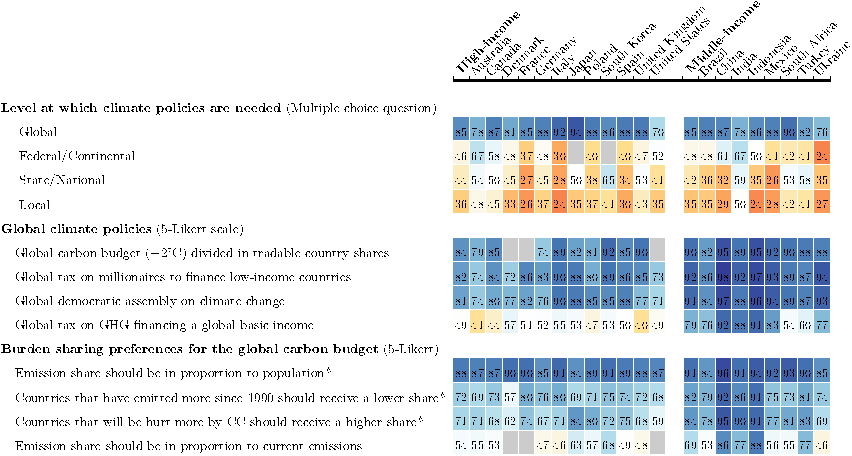
\includegraphics[width=1.2\textwidth]
  {../figures/OECD/Heatplot_global_tax_attitudes_share.pdf}}\label{fig:oecd} %
  {\footnotesize \\ $\quad$ \\ Note 1: The numbers represent the share of \textit{Somewhat} or \textit{Strongly support} among non-\textit{indifferent} answers (in percent, $n$ = 40,680). The color blue denotes a relative majority. See Figure \ref{fig:oecd_absolute} for the absolute support. (Questions \ref{q:scale}-\ref{q:millionaire_tax}%
). \\ Note 2: *In Denmark, France and the U.S., the questions with an asterisk were asked differently, cf. Question \ref{q:burden_sharing_asterisk}. } 
\end{figure}

Among the four global climate policies examined in the \textit{Global} survey, three policies garner high support across all countries (Figure \ref{fig:oecd}). These policies include a global democratic assembly on climate change, a global tax on millionaires to finance low-income countries contingent on their climate action, and a global carbon budget of +2\textdegree{}C divided among countries based on tradable shares (or ``global quota''), with the allocation of country shares unspecified.\footnote{The policies were all described with further details to make sure people understood them. Specifically, the policies were presented as follows: an international emissions trading system where ``countries that emit more than their national share would pay a fee to countries that emit less than their share''; ``a tax on all millionaires in dollars around the world to finance low-income countries that comply with international standards regarding climate action [which] would finance infrastructure and public services such as access to drinking water, healthcare, and education''; ``a global democratic assembly whose role would be to draft international treaties against climate change [where] each adult across the world would have one vote to elect members of the assembly''.} The three policies garner a majority of absolute support (i.e., ``somewhat'' or ``strong'' support) in all countries (except in the U.S. for the global assembly, 48\% absolute support). In high-income countries, the global quota policy obtains 64\% absolute support and 84\% relative support (i.e., excluding ``indifferent'' answers). %

Following the support for the global quota, respondents are asked about their preferences for dividing the carbon budget among countries, as depicted in the third block of Figure \ref{fig:oecd}. Consistent with the existing literature (see Appendix \ref{subsubsec:literature_attitudes_burden_sharing}), an equal per capita allocation of emission rights emerges as the preferred burden-sharing principle, garnering absolute majority support in all countries and never below 84\% relative support. Taking into account historical responsibilities or vulnerability to climate damages is also popular, albeit with less consensus, while grandfathering (i.e., allocation of emission shares in proportion to current emissions) receives the least support in all countries.

A global quota with equal per capita emission rights should produce the same distributional outcomes as a global carbon tax that funds a global basic income.\footnote{Similarly,  a global quota with grandfathering is equivalent to a global carbon tax where each country keeps the revenues it collects.} The support for the global carbon tax is also tested and its redistributive effects --  the average increase in expenditures along with the amount of the basic income -- are specified to the respondents explicitly  (see box below and Appendix \ref{app:questionnaire}, p. \pageref{subsec:questionnaire_GCS}). %
The support for the carbon tax is lower than for the quota, particularly in high-income countries, and there is no relative majority for the tax in Anglo-Saxon countries.\footnote{The levels of support are consistent with the findings of \citet{carattini_how_2019}, the only previous study that tested a global carbon tax.} Two possible reasons for this lower support are that distributive effects are made salient in the case of the tax, and that people may prefer a quota, perhaps because they find it more effective than a tax to reduce emissions. This interpretation is consistent with the level of support for the global quota once we make the distributive effects salient, as we do in the complementary surveys.
\subsubsection{Global Climate Scheme}\label{subsubsec:support_gcs}

The complementary surveys (\textit{US1}, \textit{US2}, \textit{Eu}) consist of a comprehensive exploration of citizens' attitudes towards the GCS. We present to respondents a detailed description of the GCS and explain its distributive effects, including specific amounts at stake (as specified in the box below). Furthermore, we assess respondents' understanding of the GCS with incentivized questions to test their comprehension of the expected financial outcome for typical individuals in high-income countries (loss) and the poorest individuals globally (gain), followed by the provision of correct answers (Figures \ref{fig:understood_each}-\ref{fig:understood_score}). %
The same approach is applied to a National Redistribution scheme (NR) targeting the top 5\% (in the U.S.) or top 1\% (in Europe) with the aim of financing cash transfers to all adults,\footnote{The wider base in the U.S. was chosen because emissions are larger in the U.S. than in Europe, and it would hardly be feasible to offset the median American's loss by taxing only the top 1\%.} calibrated to offset the monetary loss of the GCS for the median emitter in their country. We evaluate respondents' understanding that the richest would lose and the typical fellow citizens would gain from that policy. %
Subsequently, we summarize both schemes to enhance respondents' recall. Additionally, we present a final incentivized comprehension question and provide the expected answer that the combined GCS and NR would result in no net gain or loss for a typical fellow citizen. Finally, respondents are directly asked to express their support for the GCS and NR using a simple \textit{Yes}/\textit{No} question.
The stated support for the GCS is 54\% in the U.S. and 76\% in Europe,\footnote{The 95\% confidence intervals are $[52.4\%, 55.9\%]$ in the U.S. and $[74.2\%, 77.2\%]$ in Europe. The average support is computed with survey weights, employing weights based on quota variables, which exclude vote. Another method to reweigh the raw results involves running a regression of the support for the GCS on sociodemographic characteristics (including vote) and multiplying each coefficient by the population frequencies. This alternative approach yields similar figures: 76\% in Europe and 52\% or 53\% in the U.S. (depending on whether individuals who did not disclose their vote are classified as non-voters or excluded). Notably, the average support excluding non-voters is 54\% in the U.S.} while the support for NR is very similar: 56\% and 73\% respectively (see Figure \ref{fig:support_binary}). Appendix \ref{app:determinants} examines the sociodemographic determinants of support for the GCS as well as the beliefs correlated with the support for a global tax on GHG financing a global basic income. The strongest correlates are political leaning, trust in the government and perceptions that the policy is effective at reducing emissions or in one's self-interest. %

\begin{tcolorbox}\label{box:GCS}
  \paragraph{The Global Climate Scheme} The GCS consists of global emissions trading with emission rights being auctioned each year to polluting firms, and of a global basic income, funded by the auction revenues. Using the price and emissions trajectories from the report by \cite{stern_report_2017}, and in particular a carbon price of \$90/tCO$_\text{2}$ in 2030, we estimate that the basic income would amount to \$30 per month for every human over the age of 15 (see details in Appendix \ref{app:gain_gcs}). %
  We describe the GCS to the respondents as a ``climate club'' and we specify its redistributive effects: The 700 million people with less than \$2/day [in Purchasing Power Parity] would be lifted out of extreme poverty, and fossil fuel price increases would cost the typical person in their country a specified amount (see Appendix \ref{subsec:questionnaire_GCS} for details). The monthly median net cost is \$85 in the U.S., \euro{}10 in France, \euro{}25 in Germany, \euro{}5 in Spain, £20 in the UK.
\end{tcolorbox}
\setcounter{figure}{0}
\renewcommand{\thefigure}{S\arabic{figure}}
\begin{figure}[h!]
    \caption[Support for the Global Climate Scheme]{[For Supplementary Material, except first row to be included in Figure \ref{fig:support}] Support for the GCS, NR and the combination of GCS, NR and C. \\(p. \pageref{subsec:questionnaire_GCS}, Questions \ref{q:gcs_support}, \ref{q:nr_support}, \ref{q:global_tax}, \ref{q:national_tax}, and \ref{q:crg_support}).%
    }\label{fig:support_binary}
    \makebox[\textwidth][c]{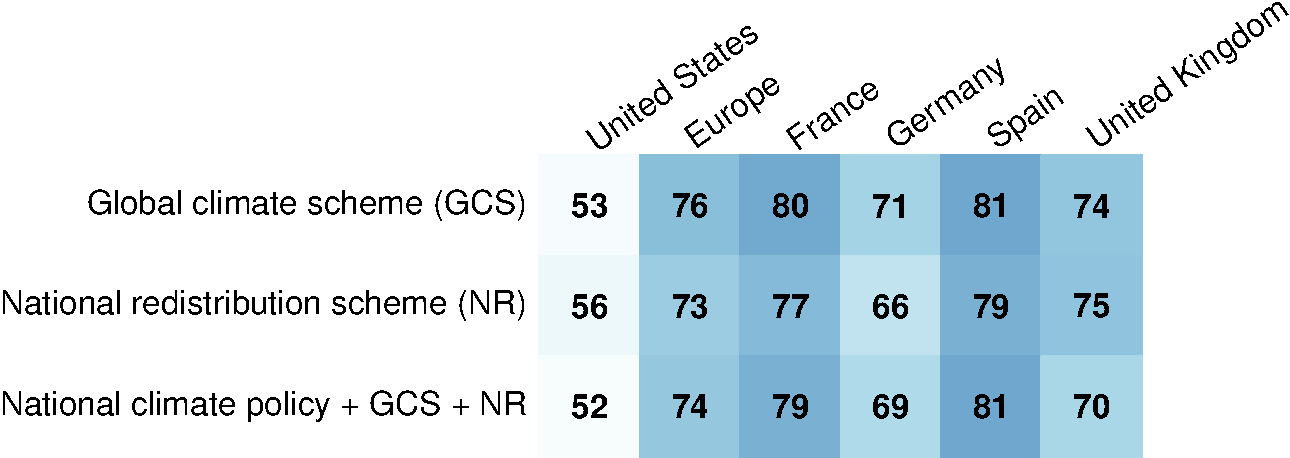
\includegraphics[width=.9\textwidth]{../figures/country_comparison/support_binary_positive.pdf}} 
\end{figure}

\subsection{Robustness and sincerity of support for the GCS}\label{subsec:robustness_sincerity}
We use several methods to assess the sincerity of the support for the GCS: a list experiment, a real-stake petition, conjoint analyses, and the prioritization of policies. All methods suggest that the support is either completely sincere, or the share of insincere answers is limited. 

\subsubsection{List experiment}\label{subsubsec:list_exp} %

By asking \textit{how many} policies within a list respondents support and varying the list among respondents, a list experiment allows identifying the tacit support for a policy of interest. The tacit support is estimated as the difference in the average number of policies supported between two groups, whose list differ only by the inclusion of that policy \citep{hainmueller_causal_2014}. %
For example, say a first subsample faces the list of policies A, B, and C, while a second subsamples faces the list A, B, C, and GCS. We do not need to know which policies each respondent support to estimate the average (tacit) support for the GCS, we simply need to compute the difference in the average number of supported policies between the two random subsamples. 
List experiments have been used to reveal social desirability bias, silencing either racism in the Southern U.S. \citep{kuklinski_racial_1997} or opposition to the invasion of Ukraine in Russia \citep{chapkovski_solid_2022}. %
In our case, as shown in Table \ref{tab:list_exp}, the tacit support for the GCS measured through the list experiment is not significantly lower than the direct stated support.\footnote{We utilize the difference-in-means estimator, and confidence intervals are computed using Monte Carlo simulation with the R package \textit{list} \citep{imai_multivariate_2011}.} Hence, we do not find a social desirability bias in our study.


\subsubsection{Petition}\label{subsubsec:petition} %

We ask respondents whether they are willing to sign a petition in support of either the GCS or NR policy. We inform them that the petition results will be sent to the head of state's office, highlighting the proportion of fellow citizens endorsing the respective scheme. Even when framed as a real-stake petition, both policies continue to receive majority support. In the U.S., we find no significant difference between the support in the real-stake petitions and the simple questions (GCS: $p=.30$; NR: $p=.76$).\footnote{Paired weighted \textit{t}-tests are conducted to test the equality in support for a policy among respondents who were questioned about the policy in the petition.} In Europe, the petition leads to a comparable lower support for both the GCS (7 p.p., $p=10^{-5}$) and NR (4 p.p., $p = .008$). While some European respondents are unwilling to sign a petition for policies they are expected to support, this effect is not specific to the GCS, and the overall willingness to sign a real-stake petition remains strong, with 69\% expressing support for the GCS and 67\% for NR.

\subsubsection{Conjoint analyses}\label{subsubsec:conjoint} %

In order to assess the public support for the GCS in conjunction with other policies, we conduct a series of conjoint analyses. We ask respondents to make five choices between pairs of political platforms.

The first conjoint analysis suggests that the GCS is supported independently of being complemented by the National Redistribution Scheme and a national climate policy (``Coal exit'' in the U.S., ``Thermal insulation plan'' in Europe, denoted C).\footnote{Indeed, 54\% of %
U.S. respondents and 74\% of %
European ones prefer the combination of C, NR and the GCS to the combination of C and NR alone, indicating similar support for the GCS conditional on NR and C than for the GCS alone (Figure \ref{fig:conjoint}).} %
For the second analysis, we split the sample into four random branches.\footnote{Results from the first branch show that the support for the GCS conditional on NR, at 55\% in the U.S. ($n$ = 757) and 77\% in Europe ($n$ = 746), is not significantly different from the support for the GCS alone. This suggests that rejection of the GCS is not driven by the cost of the policy on oneself. The second branch shows that the support for C conditional on NR is somewhat higher, at 62\% in the U.S. ($n$ = 751) and 84\% in Europe ($n$ = 747). However, the third one shows no significant preference for C compared to GCS (both conditional on NR), neither in Europe, where GCS is preferred by 52\% ($n$ = 741) nor in the U.S., where C is preferred by 53\% ($n$ = 721). The fourth branch shows that 55\% in the U.S. ($n$ = 771) and 77\% in Europe ($n$ = 766) prefer the combination of C, NR and the GCS to NR alone.} The outcome is that there is majority support for the GCS and for C, which are seen as neither complement nor substitute. A minor share of respondents like a national climate policy and dislike a global one, but as many people prefer a global rather than a national policy; and there is no evidence that implementing NR would increase the support for the GCS.
In the third analysis, we present two random branches of the sample with hypothetical progressive and conservative platforms that differ only by the presence (or not) of the GCS in the progressive platform. Table \ref{tab:conjoint_c} shows that a progressive candidate would not significantly lose voting share by endorsing the GCS in any country, and may even gain 11 p.p. ($p = .005$) in voting intention in France. %
Though the level of support for the GCS is significantly lower in swing States (at 51\%) that are key to win U.S. elections, the electoral effect of endorsing the GCS remains non-significantly different from zero (at +1.2 p.p.) in these States.\footnote{We define swing states as the 8 states with less than 5 p.p. margin of victory in the 2020 election (MI, NV, PA, WI, AZ, GA, NC, FL). The results are robust to using the 3 p.p. threshold (that excludes FL) instead.}
\begin{table}[h]
  %
  \caption[Influence of the GCS on electoral prospects]{Preference for a progressive platform depending on whether it includes the GCS or not. (Question \ref{q:conjoint_c}) 
  %
} %
  \makebox[\textwidth][c]{
\begin{tabular}{@{\extracolsep{5pt}}lcccccc} 
\\[-1.8ex]\hline 
\hline \\[-1.8ex] 
 & \multicolumn{6}{c}{Prefers the Progressive platform} \\ 
\cline{2-7} 
\\[-1.8ex] & All & United States & France & Germany & UK & Spain \\ 
\hline \\[-1.8ex] 
 GCS in Progressive platform & 0.028$^{*}$ & 0.029 & 0.112$^{***}$ & 0.015 & 0.008 & $-$0.015 \\ 
  & (0.014) & (0.022) & (0.041) & (0.033) & (0.040) & (0.038) \\ 
 \hline \\[-1.8ex] 
Constant & 0.623 & 0.604 & 0.55 & 0.7 & 0.551 & 0.775 \\ 
Observations & 5,202 & 2,619 & 605 & 813 & 661 & 504 \\ 
R$^{2}$ & 0.001 & 0.001 & 0.013 & 0.0003 & 0.0001 & 0.0003 \\ 
\hline 
\hline \\[-1.8ex] 
\end{tabular} 
}\label{tab:conjoint_c}
  {\footnotesize \textit{Note:} Simple OLS model. The 14\% of \textit{None of them} answers have been excluded from the regression samples. GCS has no significant influence on them. $^{*}p<0.1$; $^{**} p<0.05$; $^{***} p<0.01$. 
  }
\end{table}
\begin{stretchpars}
Our last two analyses  make respondents choose between two random platforms. In Europe, respondents are prompted to imagine that a left or center-left coalition will win the next election and are asked what platform they would prefer that coalition to have campaigned on. In the U.S., the question is framed as a hypothetical duel in a Democratic primary, and asked only to non-Republicans ($n$ = 2,218), i.e. the respondents who declare as political affiliation \textit{Democrat}, \textit{Independent}, \textit{Non-Affiliated} or \textit{Other}. In the fourth analysis, a policy (or an absence of policy) is randomly drawn for each platform in each of five categories: \textit{economic issues}, \textit{societal issues}, \textit{climate policy}, \textit{tax system}, \textit{foreign policy} (Figure \ref{fig:ca_r}). 

Except for the category \textit{foreign policy}, which features the GCS 42\% of the time, the policies are prominent progressive policies and they are drawn uniformly. %
In the UK, Germany, and France, a platform is about 9 to 13 p.p. more likely to be preferred if it includes the GCS rather than no foreign policy.\footnote{This is the Average Marginal Component Effect computed following \citet{hainmueller_causal_2014}.} This effect is between 1 and 4 p.p. and no longer significant in the U.S. and in Spain. Moreover, a platform that includes a global tax on millionaires rather than no foreign policy is 5 to 13 percentage points (p.p.) more likely to be preferred in all countries (the effect is significant and at least 9 p.p. in all countries but Spain). 
Similarly, a global democratic assembly on climate change has a significant effect of 8 to 12 p.p. in the U.S., Germany, and France. 
These effects are large, and not far from the effects of the policies most influential on the platforms, which range between 15 and 18 p.p. in most countries (and 27 p.p. in Spain), and all relate to improved public services (in particular healthcare, housing, and education).
\end{stretchpars}
 
\begin{figure}[h] 
  \caption[Preferences for various policies in political platforms]{[For Supplementary Material] Effects of the presence of a policy (rather than none from this domain) in a random platform on the likelihood that it is preferred to another random platform. (See English translations in Figure \ref{fig:ca_r_en}; Question \ref{q:conjoint_r}%
  )}\label{fig:ca_r}
  \begin{subfigure}{\textwidth}
    \subcaption{U.S. (Asked only to non-Republicans)}
    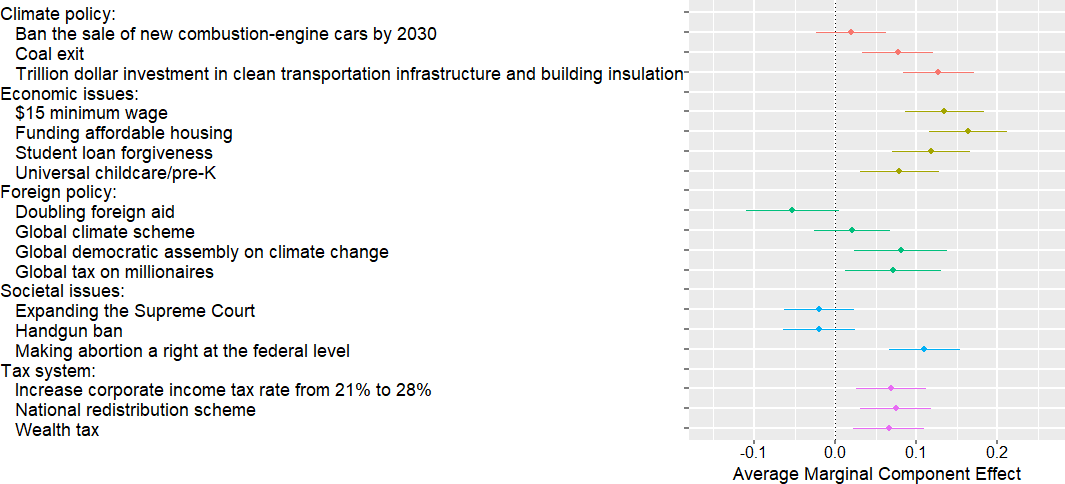
\includegraphics[width=\textwidth]{../figures/US1/ca_r.png}
  \end{subfigure}
  \begin{subfigure}{\textwidth}
    \subcaption{France}
    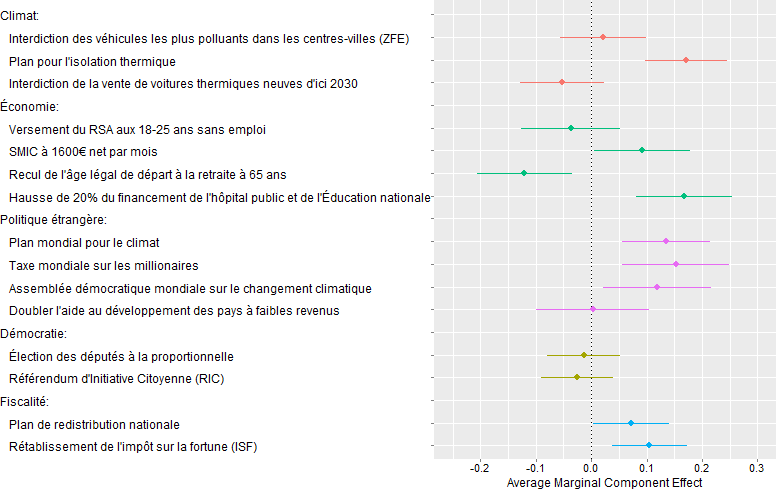
\includegraphics[width=\textwidth]{../figures/FR/ca_r.png}
  \end{subfigure}
\end{figure}%
\clearpage
\begin{figure}[h!]\ContinuedFloat %
  \begin{subfigure}{\textwidth}
    \subcaption{Germany}
    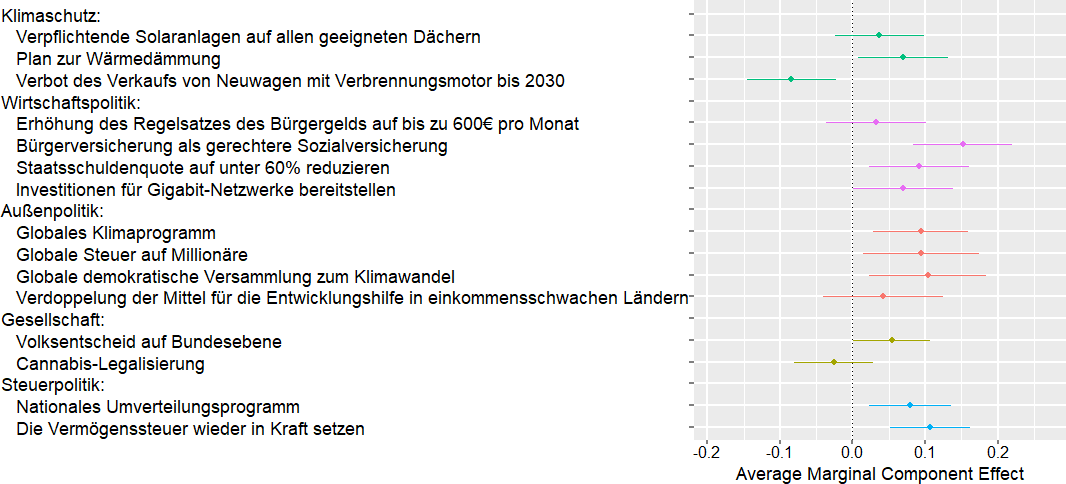
\includegraphics[width=\textwidth]{../figures/DE/ca_r.png}
  \end{subfigure}
  \begin{subfigure}{\textwidth}
    \subcaption{Spain}
    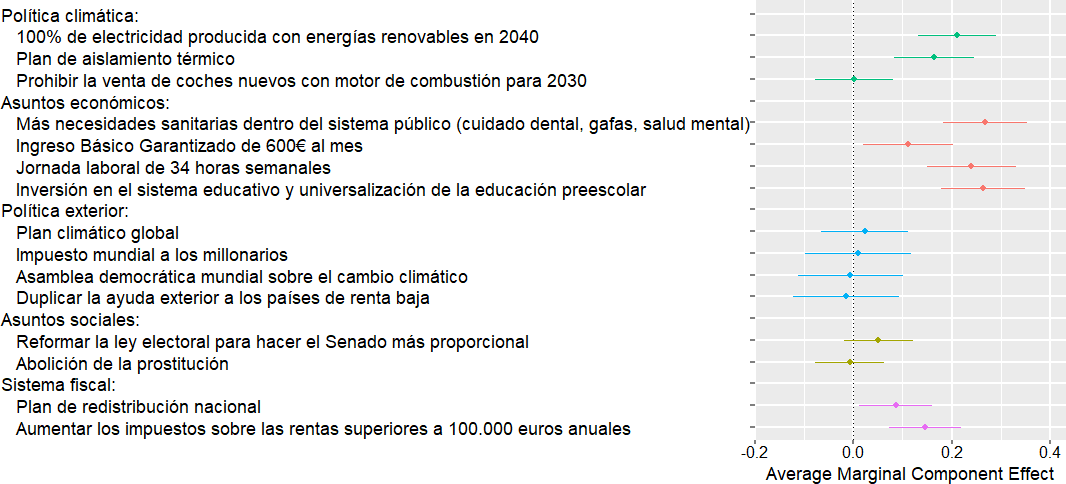
\includegraphics[width=\textwidth]{../figures/ES/ca_r.png}
  \end{subfigure}
  \begin{subfigure}{\textwidth}
    \subcaption{UK}
    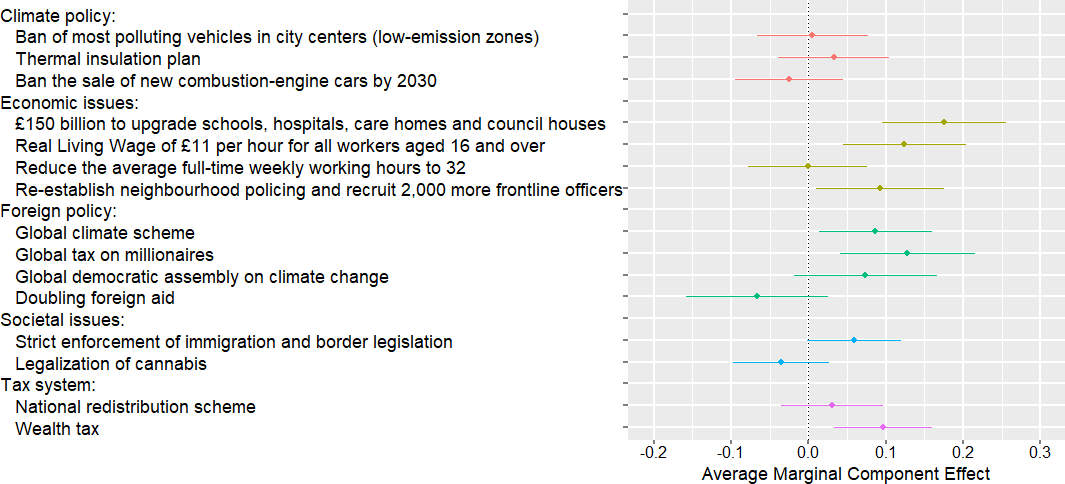
\includegraphics[width=\textwidth]{../figures/UK/ca_r.png}
  \end{subfigure}
  %
\end{figure}
\clearpage 
\noindent 
The fifth analysis draws random platforms similarly, except that candidate A's platform always contains the GCS while B's includes no foreign policy. In this case, A is chosen by 60\% in Europe %
and 58\% in the U.S. (Figure \ref{fig:conjoint_left_ag_b}). %
Overall, taking the U.S. as an example, our conjoint analyses indicate that a candidate at the Democratic primary would have more chances to obtain the nomination by endorsing the GCS, and this endorsement would not penalize her or him at the presidential election. This result reminds the finding that 12\% of Germans shift their voting intention from SPD and CDU/CSU to the Greens and the Left when they are told that the latter parties support global democracy \citep{ghassim_who_2020}.
\begin{figure}[h!]
    \caption[Influence of the GCS on preferred platform]{[For Supplementary Material] Influence of the GCS on preferred platform:\\ Preference for a random platform A that contains the Global Climate Scheme rather than a platform B that does not (in percent). (Question \ref{q:conjoint_d}; in the U.S., asked only to non-Republicans.)}\label{fig:conjoint_left_ag_b}
    \makebox[\textwidth][c]{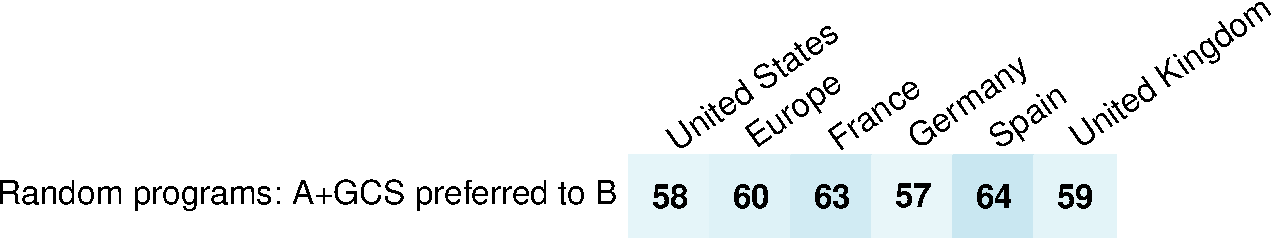
\includegraphics[width=\textwidth]{../figures/country_comparison/conjoint_left_ag_b_binary_positive.pdf}} 
\end{figure}
\subsubsection{Prioritization}\label{subsubsec:prioritization} %

Towards the end of the survey, we ask respondents to allocate 100 points among six randomly selected policies from the previous conjoint analyses, using sliders. The instruction was to distribute the points based on their level of support, with a higher allocation indicating greater support for a policy. %
As a result, the average support across policies is 16.67 points. %
In each country, the GCS ranks in the middle of all policies or above, with an average number of points from 15.4 in the U.S. to 22.9 in Germany.%

Interestingly, in Germany, the most prioritized policy is the global tax on millionaires, while the GCS is the second most prioritized policy. The global tax on millionaires consistently ranks no lower than fifth position (out of 15 or 17 policies) in every country, garnering an average of 18.3 points in Spain to 22.9 points in Germany.

This question sheds light on a potential discrepancy between the policy priorities of the public and those enacted by legislators. For instance, while the European Union and California have enacted plans to phase out new combustion-engine cars by 2035, the proposal to ``ban the sale of new combustion-engine cars by 2030'' emerged as one of the three least prioritized policies in each country, with an average allocation of 7.8 points in France to 11.4 points in the UK.

  
\subsubsection{Pros and Cons}\label{subsubsec:pros_cons}

We survey respondents to gather their perspectives on the pros and cons of the GCS, utilizing either an open-ended or a closed question. In the closed question format, respondents tend to consider every argument as important in determining their support or opposition to the GCS (see Figure \ref{fig:gcs_important}). Notably, the least important aspect was the negative impact on their household, with 60\% in Europe ($n$=1,505) and 75\% in the U.S. ($n$=493) finding it important. The most important elements differ between Europe and the U.S. In Europe, the key factors are the GCS's potential to limit climate change and reduce poverty in low-income countries, both deemed important by 85\% of respondents. In the U.S., having sufficient information about the scheme ranks highest at 89\%, followed by its potential to foster global cooperation at 82\%. However, due to the limited variation in the ratings for each element, the closed question format is inconclusive (Figure \ref{fig:gcs_important}). %

The open-ended question provides more insights into what people associate with the GCS when prompted to think about it. %
Analyzing keywords in the responses (automatically translated into English), the most frequently mentioned topics are the international aspect and the environment, each appearing in approximately one-quarter of the answers (see Figure \ref{fig:gcs_field_contains}). This is followed by discussions on the effects of the GCS on poverty and prices, each mentioned by about one-tenth of the respondents. We also manually classified each answer into different categories (see Figure \ref{fig:gcs_field}). This exercise confirms the findings from the automatic search: the environmental benefit of the GCS is the most commonly discussed topic, while obstacles to implementation or agreement on the proposal are relatively infrequently mentioned.%
\footnote{Moreover, around one in four respondents explicitly cites pros or cons. Few individuals explicitly express support or opposition, and misunderstandings are rare. Only 11\% of the responses are empty or express a lack of opinion, though one-quarter are unclassifiable due to the rarity, nonsensical nature, or irrelevance of the conveyed idea.}%

In the \textit{US2} survey, we divided the sample into four random branches. 
Two branches were presented the pros and cons questions (either in open or closed format) \textit{before} being asked about their support for the GCS or NR. Another branch received information on the actual level of support for the GCS and NR (estimated in \textit{US1}, see Section \ref{subsec:second_order_beliefs}), and one control group received none of these treatments. %
The objective of this ``pros and cons treatment'' was to simulate a ``campaign effect'', which refers to the shift in opinion resulting from media coverage of the proposal. To conservatively estimate the effect of a (potentially negative) campaign, we intentionally included more cons (6) than pros (3). Interestingly, the support for the GCS decreased by 11 p.p. after respondents viewed a list of its pros and cons.\footnote{Surprisingly, the support for National Redistribution also decreased by 7 p.p. following the closed question about the GCS. This suggests that some individuals may lack attention and confuse the two policies, or that contemplating the pros and cons alters the mood of some people, moving them away from their initial positive impression.} Notably, the support also decreased by 7 p.p. after respondents were asked to consider the pros and cons in an open-ended question. Although support remains significant,%
\footnote{Despite some significant effects of pondering the pros and cons, approximately half of the Americans express support for the GCS across all treatment branches (see Table \ref{tab:branch_gcs}).} 
these results suggest that the public success of the GCS would be sensitive to the content of the debate about it, and subject to the discourse adopted by interest groups. %

\subsection{Second-order Beliefs}\label{subsec:second_order_beliefs}
To explain the strong support for the GCS despite its absence from political platforms and public debate, 
we hypothesized pluralistic ignorance, i.e. that the public and policymakers mistakenly perceive the GCS as unpopular. As a result, individuals might conceal their support for such globally redistributive policies, believing that advocating for them would be futile. 
However, the evidence for pluralistic ignorance is limited based on an incentivized question about perceived support (Figure \ref{fig:belief}).

In the case of Americans, 
their beliefs about the level of support for the GCS are relatively accurate. The mean perceived support is 52\% (with quartiles of 36\%, 52\%, and 68\%), which closely aligns with the actual support of 53\%. Europeans, on the other hand, underestimate the support by 17 p.p. Nonetheless, 65\% of them correctly estimate that the GCS garners majority support, and the mean perceived support is 59\% (and quartiles of 43\%, 61\%, and 74\%), compared to the actual support of 76\%. 
Second-order beliefs are equally accurate for NR in the U.S. and similarly underestimated in Europe. %
Finally, consistent with Americans accurately perceiving the levels of support for the GCS or NR, providing information on the actual level had no significant effect on their support in the \textit{US2} survey. %

\begin{figure}[h!]
    \caption[Beliefs about support for the GCS and NR]{[For Supplementary Material] Beliefs regarding the support for the GCS and NR. (Questions \ref{q:gcs_belief} and \ref{q:nr_belief})}\label{fig:belief}
    \makebox[\textwidth][c]{
\includegraphics[width=.7\textwidth]{../figures/country_comparison/belief_all_mean.pdf}} 
\end{figure}

\subsubsection{Other global policies}\label{subsubsec:support_other_global_policies} %

We also assess support for other global policies (Figure \ref{fig:support}). 
Most policies garner relative majority support in each country, with two exceptions: 
the ``cancellation of low-income countries' public debt'' and ``a maximum wealth limit'' for each individual. 
The latter policy obtains relative majority support in Europe but not in the U.S., despite the cap being set at \$10 billion in the U.S. compared to \euro{}/£100 million in Europe. Notably, climate-related policies enjoy significant popularity, with ``high-income countries funding renewable energy in low-income countries'' receiving absolute majority support across all surveyed countries. Additionally, relative support for loss and damages compensation, as approved in principle at the international climate negotiations in 2022 (``COP27''), ranges from 55\% (U.S.) to 81\% (Spain), with absolute support ranging from 41\% to 62\%.

\subsubsection{Global wealth tax}\label{subsubsec:support_global_wealth_tax}

Consistent with the results of the global survey, a ``tax on millionaires of all countries to finance low-income countries'' garners absolute majority support of over 67\% in each country, only 5 p.p. lower than a national millionaires tax overall (Figure \ref{fig:support}). In random subsamples, we inquire about respondents' preferences regarding the redistribution of revenues from a global tax on individual wealth exceeding \$5 million, after providing information on the revenue raised by such a tax in their country compared to low-income countries.\footnote{A 2\% tax on net wealth exceeding \$5 million would annually raise \$816 billion, leaving unaffected 99.9\% of the world population. More specifically, it would collect \euro{}5 billion in Spain, \euro{}16 billion in France, £20 billion in the UK, \euro{}44 billion in Germany, \$430 billion in the U.S., and \$1 billion collectively in all low-income countries (28 countries, home to 700 million people).%
} We ask certain respondents ($n$ = 1,283) what percentage of global tax revenues should be pooled to finance low-income countries. In each country, at least 88\% of respondents indicate a positive amount, with an average ranging from 30\% (Germany) to 36\% (U.S., France) (Figure \ref{fig:global_share_mean}). To other respondents ($n$ = 1,233), we inquire whether they would prefer each country to retain all the revenues it collects or that half of the revenues be pooled to finance low-income countries. Approximately half of the respondents opt to allocate half of the tax revenues to low-income countries.
\begin{figure}
    \centering 
    \caption[Preferred share of wealth tax for low-income countries]{[For Supplementary Material] Percent of global wealth tax that should finance low-income countries (\textit{mean}). (Question \ref{q:global_tax_global_share})} %
    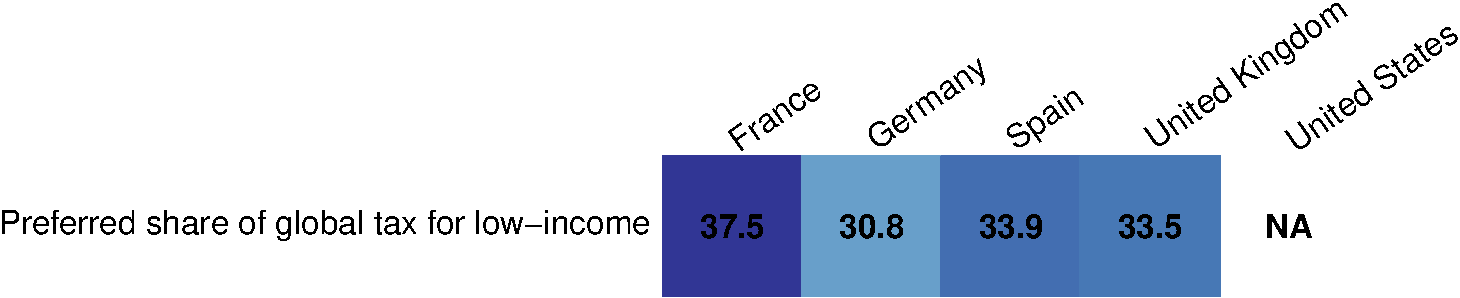
\includegraphics[width=1\textwidth]{../figures/country_comparison/global_tax_global_share_mean.pdf} \label{fig:global_share_mean}
\end{figure}


\setcounter{figure}{1}
\renewcommand{\thefigure}{\arabic{figure}}
\begin{figure}
  %
  \caption[Relative support for further global policies]{Relative support for various global policies (percentage of \textit{somewhat} or \textit{strong support}, after excluding \textit{indifferent} answers). (Questions \ref{q:climate_policies} and \ref{q:other_policies}; See Figure \ref{fig:support_likert_positive} for the absolute support.)%
  }
  \makebox[\textwidth][c]{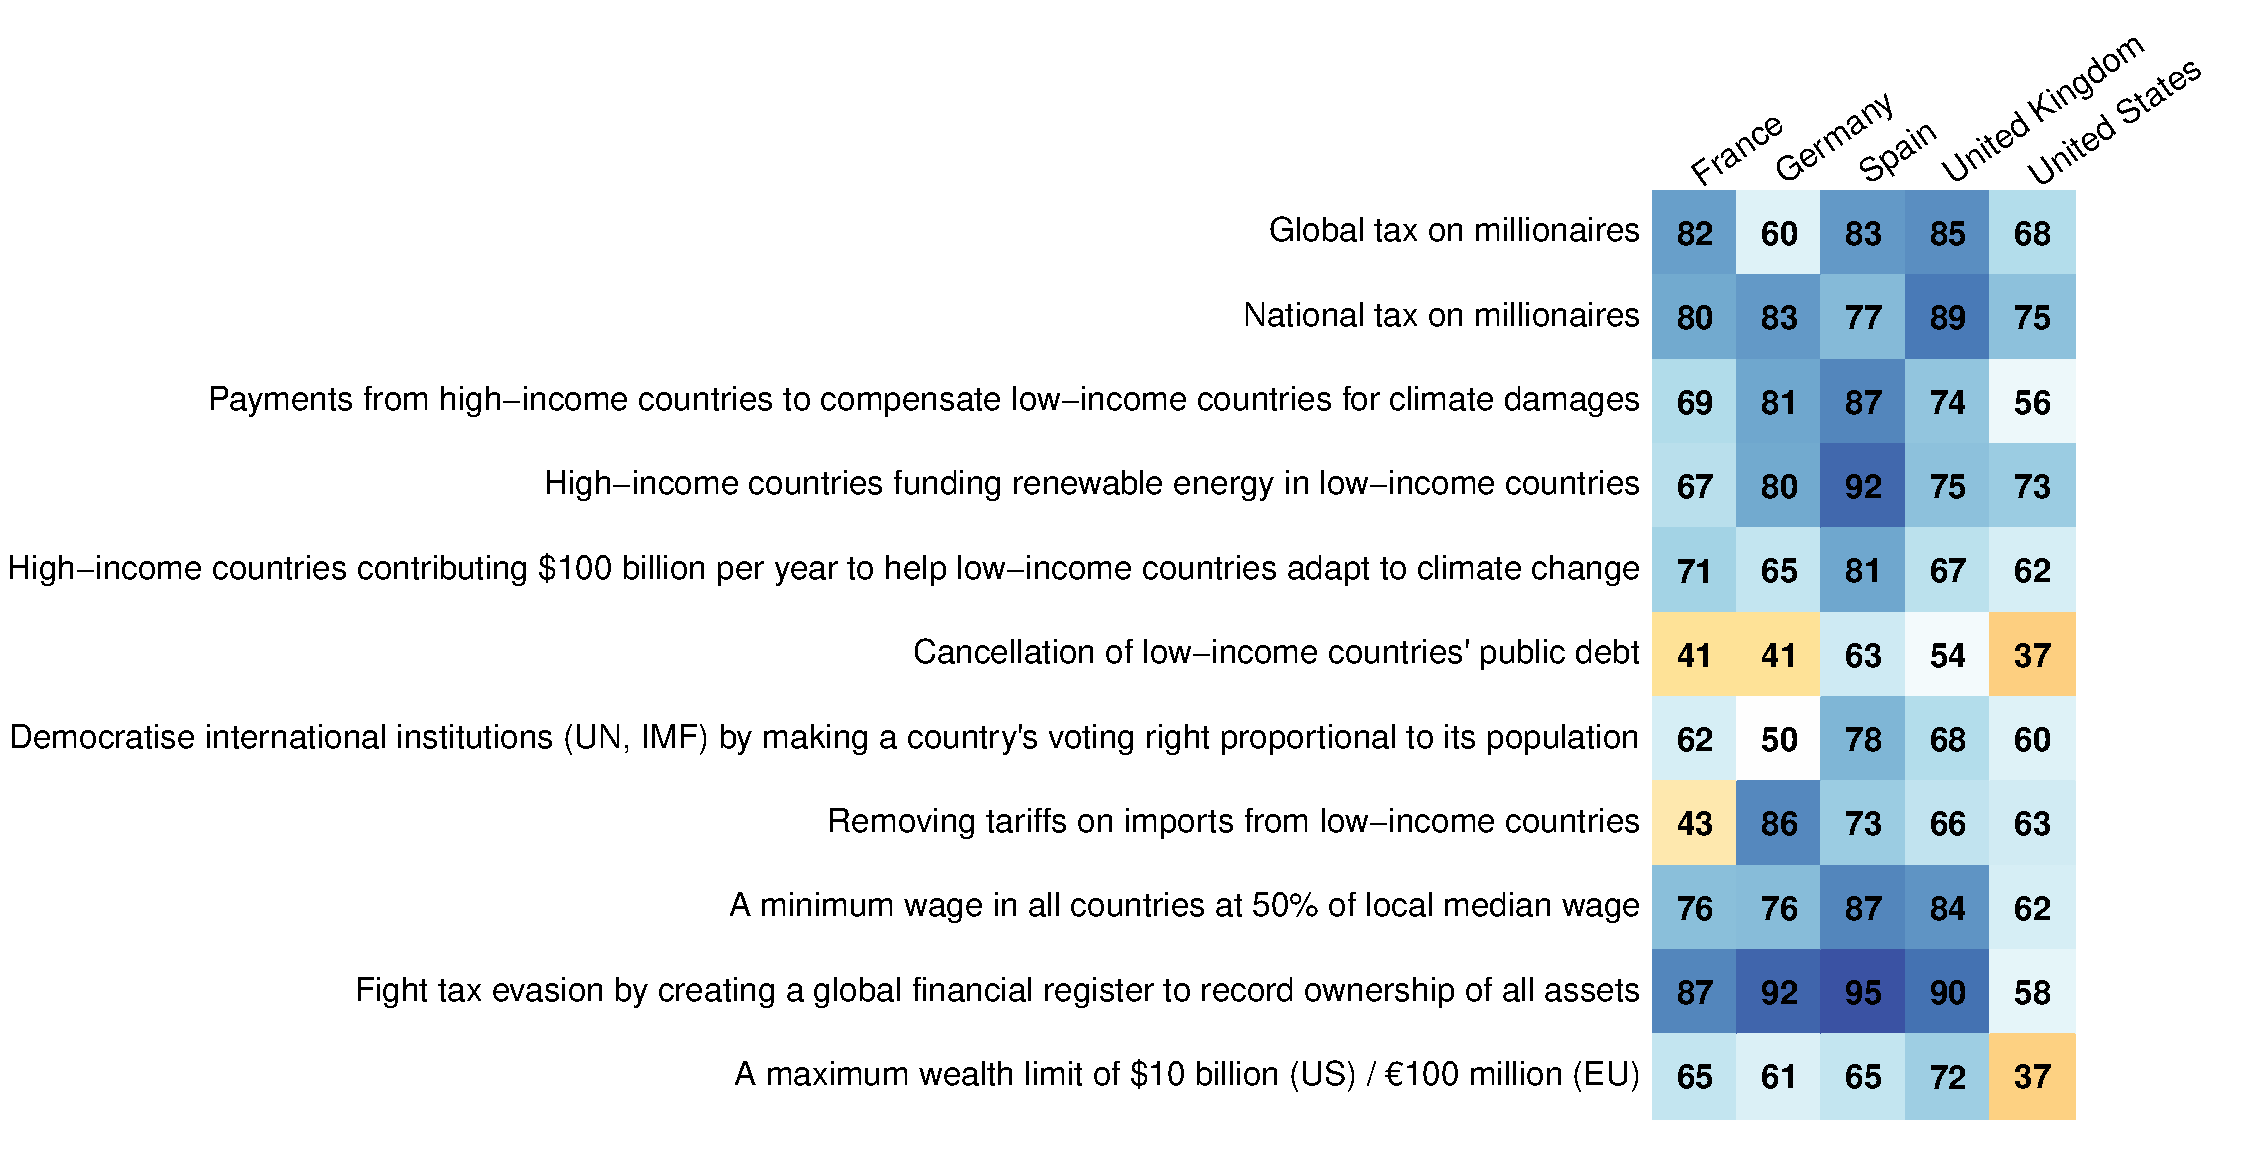
\includegraphics[width=\textwidth]{../figures/country_comparison/support_likert_share.pdf}}\label{fig:support}
\end{figure} 
\renewcommand{\thefigure}{S\arabic{figure}}

\subsubsection{Foreign aid}\label{subsubsec:support_foreign_aid} %

We provide respondents with information about the actual amount ``spent on foreign aid to reduce poverty in low-income countries'' relative to their country's government spending and GDP. Less than 16\% of respondents state that their country's foreign aid should be reduced, while 62\% express support for increasing it, including 17\% who support an unconditional increase (Figure \ref{fig:foreign_aid_raise_support}). Among the 45\% who think aid should be increased under certain conditions, we subsequently ask them to specify the conditions they deem necessary (Figure \ref{fig:foreign_aid_condition}). The three most commonly selected conditions are: ``we can be sure the aid reaches people in need and money is not diverted'' (73\% chose this condition), ``that recipient countries comply with climate targets and human rights'' (67\%), and ``that other high-income countries also increase their foreign aid'' (48\%).\footnote{It is worth noting that these conditions align closely with the principles of the GCS.} 
On the other hand, respondents who do not wish to increase their country's foreign aid primarily justify their view by prioritizing the well-being of their fellow citizens or by perceiving each country as responsible for its own fate (Figure \ref{fig:foreign_aid_no}). In response to an open-ended question regarding measures high-income countries should take to fight extreme poverty, a large majority of Americans expressed that more help is needed (Figure \ref{fig:poverty_field}). The most commonly suggested form of aid is financial support, closely followed by investments in education. 
We also inquire about the perceived amount of foreign aid. Consistent with prior research (see Appendix \ref{subsubsec:literature_foreign_aid}), most people overestimate the actual amount of foreign aid (Figure \ref{fig:foreign_aid_belief}). We then elicit respondents' preferred amount of foreign aid, after randomly presenting them with either the actual amount or no information. Most of the respondents who learn the actual amount choose a bracket at least as high as the actual one, and most of those without the information choose a bracket at least as high as the perceived one (Figures \ref{fig:foreign_aid_amount}--\ref{fig:foreign_aid_preferred_info}). Finally, we ask a last question to the respondents who received the information. To those who prefer an increase of foreign aid, we ask how they would finance it: by far, the preferred source of funding is higher taxes on the wealthiest (Figure \ref{fig:foreign_aid_raise_how}). To those who prefer a reduction, we ask how they would use the funds becoming available: %
In every country, more people choose higher spending on education or healthcare rather than lower taxes (Figure \ref{fig:foreign_aid_reduce_how}). 

\begin{figure}[h!]
  \caption[Attitudes on the evolution of foreign aid]{[For Supplementary Material] Attitudes regarding the evolution of [own country] foreign aid. (Question \ref{q:foreign_aid_raise_support})}\label{fig:foreign_aid_raise_support}
  \makebox[\textwidth][c]{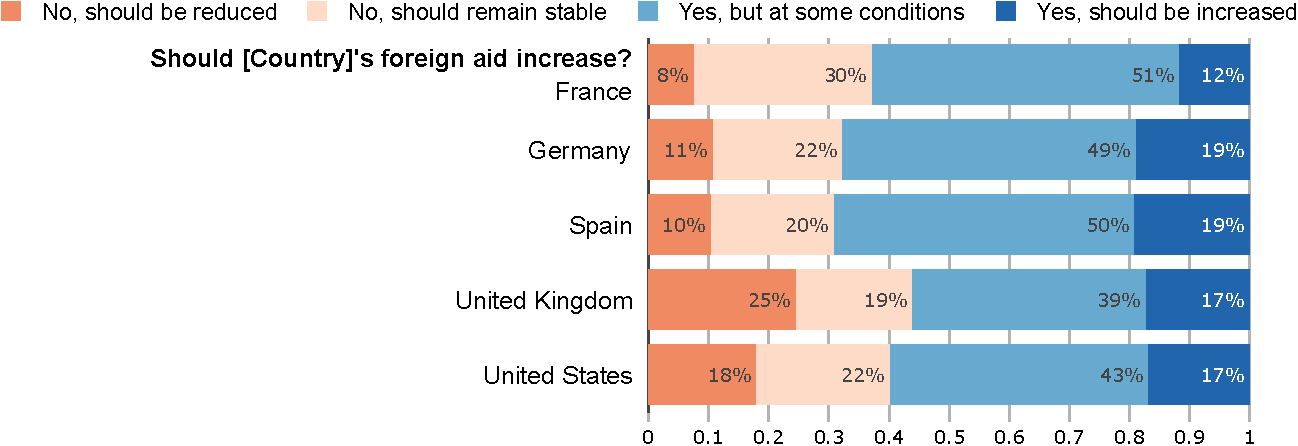
\includegraphics[width=\textwidth]{../figures/country_comparison/foreign_aid_raise_support.pdf}} 
\end{figure}

\begin{figure}[h!]
  \caption[Conditions at which foreign aid should be increased]{[For Supplementary Material] Conditions at which foreign aid should be increased (in percent). [Asked to those who wish an increase of foreign aid at some conditions.] (Question \ref{q:foreign_aid_condition})}\label{fig:foreign_aid_condition}
  \makebox[\textwidth][c]{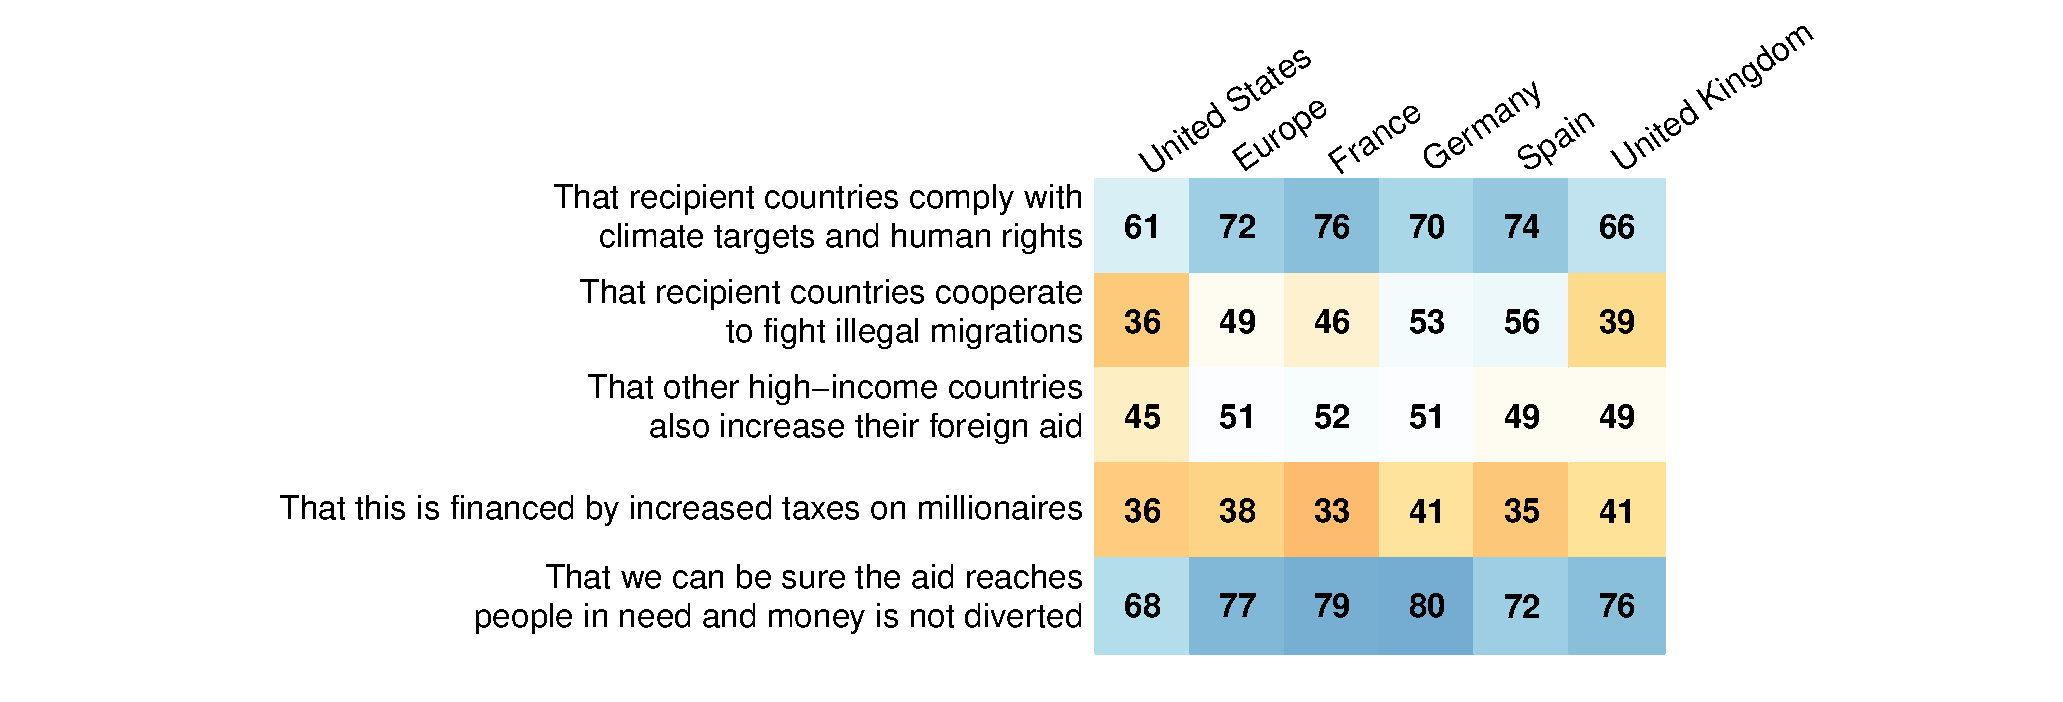
\includegraphics[width=\textwidth]{../figures/country_comparison/foreign_aid_condition_positive.pdf}} 
\end{figure}

\begin{figure}[h!]
  \caption[Reasons why foreign aid should not be increased]{[For Supplementary Material] Reasons why foreign aid should not be increased (in percent). [Asked to those who wish a decrease or stability of foreign aid.] (Question \ref{q:foreign_aid_no})}\label{fig:foreign_aid_no}
  \makebox[\textwidth][c]{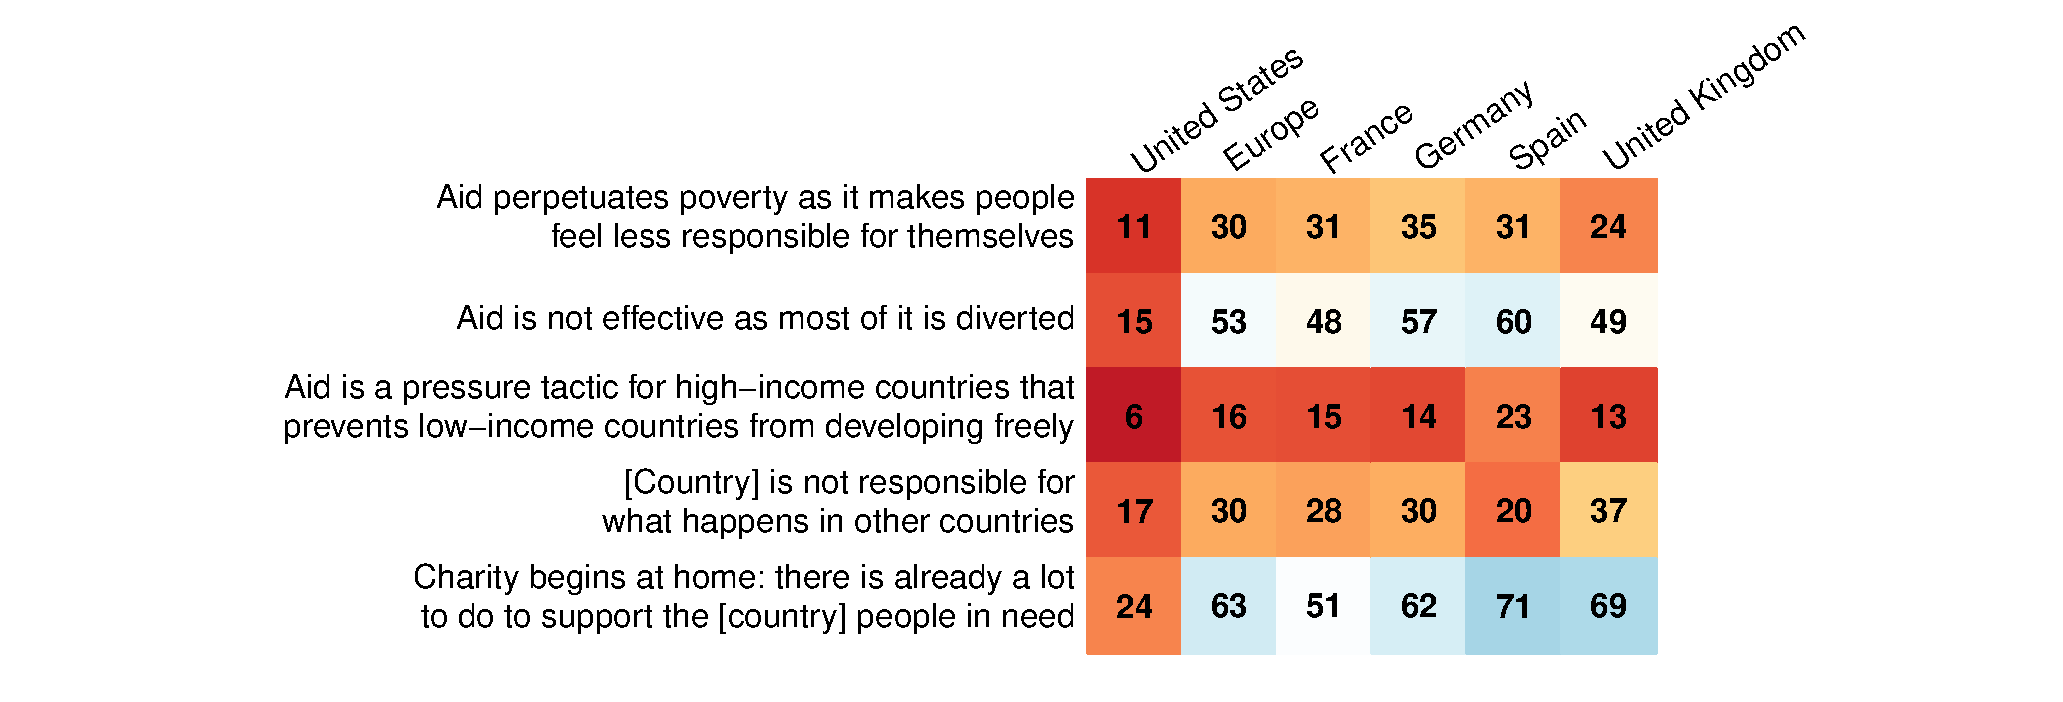
\includegraphics[width=\textwidth]{../figures/country_comparison/foreign_aid_no_positive.pdf}} 
\end{figure}

\subsection{Universalistic values}\label{subsec:universalistic}

We also elicit underlying values, to test whether broad values are consistent with people's support for specific policies. %
When we ask respondents which group they defend when they vote, %
20\% choose ``sentient beings (humans and animals),'' 22\% choose ``humans,'' 33\% select their ``fellow citizens'' (or ``Europeans''), 15\% choose ``My family and myself,'' and the remaining 10\% choose another group (mainly ``My State or region'' or ``People sharing my culture or religion''). The first two categories, representing close to one out of two people, can be described as universalist in their vote. Notably,  a majority of left-wing voters can even be considered universalist voters (see Figure \ref{fig:main_by_vote} for main attitudes by vote).%

When asked what their country's diplomats should defend in international climate negotiations, only 11\% prefer their country's ``interests, even if it goes against global justice.'' In contrast, 30\% prefer global justice (with or without consideration of national interests), and the bulk of respondents (38\%) prefer their country's ``interests, to the extent it respects global justice.''

Furthermore, when we ask respondents to assess the extent to which climate change, global poverty, and inequality in their country are issues, climate change is generally viewed as the most significant problem (with a mean score of 0.59 after recoding answers between -2 and 2). This is followed by global poverty (0.42) and national inequality (0.37). %

Finally, we conduct a lottery experiment to elicit universalistic values. Respondents were automatically enrolled in a lottery with a \$100 prize and had to choose the proportion of the prize they would keep for themselves versus give to a person living in poverty. The charity donation is directed either to an African individual or a fellow citizen, depending on the respondent's random assignment. In Europe, we observe no significant variation in the willingness to donate based on the recipient's origin. In the U.S., the donations to Africans are 3 p.p. lower (with an average donation of 34\%), but the slightly lower donations to Africans are entirely driven by Trump voters and non-voters (Table \ref{tab:donation}).

Overall, answers to these broad value questions are consistent with half of Americans and three quarters of Europeans supporting global policies like the GCS: people are almost as much willing to give to poor Africans than to poor fellow citizens, find that global issues are among the biggest problems, almost half of them are universalist when they vote, and most of them wish that their diplomats take into account global justice.

\section{Discussion} %
Our point of departure are recent surveys conducted %
in 20 of the largest countries%
, as they reveal robust majority support for global redistributive and climate policies, even in high-income countries that would financially lose from them. The results from complementary surveys conducted in the U.S. and four European countries %
reinforce these findings. We find strong support for global taxes on the wealthiest individuals, as well as majority support for our main policy of interest -- the Global Climate Scheme (GCS). The GCS encompasses carbon pricing at a global level through an emissions trading system, accompanied by a global basic income funded by the scheme's revenues. Additional experiments, such as a list experiment and a real-stake petition, demonstrate that the support for the GCS is real. 
Such genuine support is further substantiated by the prioritization of the GCS over prominent national climate policies and aligned with a significant portion of the population holding universalistic values rather than nationalistic or egoistic ones. Moreover, the conjoint analyses indicate that a progressive candidate would not lose voting shares by endorsing the GCS, and may even gain 11 p.p. in voting shares in France. Similarly, a candidate endorsing the GCS would gain votes in a U.S. Democratic primary, while in Europe, a progressive platform that includes the GCS would be preferred over one that does not.

Having ruled out insincerity and underestimation of fellow citizens' support as potential explanations for the scarcity of global policies in the public debate, we propose alternative explanations. %
The first two are variations of pluralistic ignorance, and the last three represent complementary explanations. 

First, there may be pluralistic ignorance \textit{among policymakers} regarding universalistic values, support for the GCS, or the electoral advantage of endorsing it. Second, people or policymakers may believe that globally redistributive policies are politically infeasible in some key (potentially foreign) countries like the U.S. %
Third, political discourse centrally happens at the national level, shaped by national media and institutions such as voting. 
National framing by political voices may create biases and suppress universalistic values. %
Fourth, many individuals, including policymakers, may perceive global redistributive policies as ill-defined or technically infeasible, ultimately dismissing them as unrealistic. In particular, policymakers may have insider information about the technical feasibility of such policies. Alternatively, the perception of unrealism may stem from an unawareness of specific proposals. %
Fifth, just as policy is disproportionately influenced by the economic elites \citep{gilens_testing_2014,persson_rich_2023}, public debate may be shaped by the wealthiest, who have vested interests in preventing global redistribution.

Confirmation of any of these hypotheses would lead to a common conclusion: there exists substantial support for global policies addressing climate change and global inequality, even in high-income countries, and the perceived boundaries of political realism on this issue may soon shift. %
Uncovering evidence to support the above hypotheses could %
draw attention to global policies in the public debate and contribute to their increased prominence. %
  \begin{small} %
\section*{\normalsize Methods}\label{sec:methods} %
\addcontentsline{toc}{section}{\nameref{sec:methods}}
\paragraph{\small Data collection.} %

The paper utilizes two sets of surveys: the \textit{Global} survey and the \textit{Complementary} surveys. The \textit{Complementary} surveys consist of two U.S. surveys, \textit{US1} and \textit{US2}, and one European survey, \textit{Eu}. The \textit{Global} survey was conducted from March 2021 to March 2022 on 40,680 respondents from 20 countries (with 1,465 to 2,488 respondents per country). \textit{US1} collected responses from 3,000 respondents between January and March 2023, while \textit{US2} gathered data from 2,000 respondents between March and April 2023. \textit{Eu} included 3,000 respondents and was conducted from February to March 2023. We used the survey companies \emph{Dynata} and \emph{Respondi}. To ensure representative samples, we employed stratified quotas based on gender, age (5 brackets), income (4), region (4), education level (3), and ethnicity (3) for the U.S. We also incorporated survey weights throughout the analysis to account for any remaining imbalances. These weights were constructed using the quota variables as well as the degree of urbanity, and trimmed between 0.25 and 4. By applying weights, the results are fully representative of the respective countries. Results at the European level apply different weights which ensure  representativeness of the combined four European countries. Appendix \ref{app:representativeness} confirms that our samples are representative of the population. %
Appendix \ref{app:balance} shows that the treatment branches are balanced. Appendix \ref{app:placebo} runs placebo tests of the effects of each treatment on unrelated outcomes. We do not find effects of earlier treatments on unrelated outcomes arriving later in the survey.
\paragraph{\small Data quality.} %
The median duration is 28 minutes for the \textit{Global} survey, 14 min for \textit{US1}, 11 min for \textit{US2}, and 20 min for \textit{Eu}. To ensure the best possible data quality, we exclude respondents who fail an attention test or rush through the survey (i.e., answer in less than 11.5 minutes in the \textit{Global} survey, 4 minutes in \textit{US1} or \textit{US2}, 6 minutes in \textit{Eu}). %

\paragraph{\small Questionnaires and raw results.} %
The questionnaire and raw results of the \textit{Global} survey can be found in the Appendix of the companion paper \citep{dechezlepretre_fighting_2022}. %
The raw results are reported in Appendix \ref{app:raw_results}\footnote{Country-specific raw results are also available as supplementary material files:  \href{https://github.com/bixiou/international_attitudes_toward_global_policies/raw/main/paper/app_desc_stats_US.pdf}{US}, \href{https://github.com/bixiou/international_attitudes_toward_global_policies/raw/main/paper/app_desc_stats_EU.pdf}{EU}, \href{https://github.com/bixiou/international_attitudes_toward_global_policies/raw/main/paper/app_desc_stats_FR.pdf}{FR}, \href{https://github.com/bixiou/international_attitudes_toward_global_policies/raw/main/paper/app_desc_stats_DE.pdf}{DE}, \href{https://github.com/bixiou/international_attitudes_toward_global_policies/raw/main/paper/app_desc_stats_ES.pdf}{ES}, \href{https://github.com/bixiou/international_attitudes_toward_global_policies/raw/main/paper/app_desc_stats_UK.pdf}{UK}.} while the surveys' structures and questionnaires are given in Appendices \ref{app:questionnaire_oecd} and \ref{app:questionnaire}. The questionnaires are the same as the ones given \textit{ex ante} in the registration plan (\href{https://osf.io/fy6gd}{osf.io/fy6gd}).
\paragraph{\small Incentives.} %
To encourage accurate and truthful responses, several questions of the \textit{US1} survey use incentives. For each of the three comprehension questions that follow the policy descriptions, we randomly select and reward three respondents who provide correct answers with a \$50 gift certificate. Similarly, for questions involving estimating support shares for the GCS and NR, three respondents with the closest guesses to the actual values receive a \$50 gift certificate. In the donation lottery question, we randomly select one respondent and split the \$100 prize between the NGO GiveDirectly and the winner according to the winner's choice. In total, our incentives scheme distributes gift certificates (and donations) for a value of \$850. Finally, respondents have an incentive to answer truthfully to the petition question, as they are aware that the results for that question (the share of respondents supporting the policy) will be transmitted to the U.S. President's office.
\section*{\normalsize Data and code availability}

All data and code of the \textit{Complementary} surveys as well as figures of the paper are available on \href{https://github.com/bixiou/international_attitudes_toward_global_policies}{github.com/bixiou/global\_tax\_attitudes}. Data and code for the \textit{Global} survey will be made public upon publication. %

\begin{table}[h]
  %
  %
  \caption[List experiment: tacit support for the GCS]{Number of supported policies in the list experiment depending on the presence of the Global Climate Scheme (GCS) in the list. %
   The tacit support for the GCS is estimated by regressing the number of supported policies on the presence of the GCS in the list of policies. The social desirability is estimated as the difference between the tacit and stated support, and it is not significantly different from zero even at a 20\% threshold (see \nameref{sec:methods}).
  }\label{tab:list_exp}
  \makebox[\textwidth][c]{
\begin{tabular}{@{\extracolsep{5pt}}lccc} 
\\[-1.8ex]\hline 
\hline \\[-1.8ex] 
 & \multicolumn{3}{c}{Number of supported policies} \\ 
\cline{2-4} 
\\[-1.8ex] & All & US & Europe \\ 
\hline \\[-1.8ex] 
 List contains: GCS & 0.624$^{***}$ & 0.524$^{***}$ & 0.724$^{***}$ \\ 
  & (0.028) & (0.041) & (0.036) \\ 
\hline  \\[-1.8ex] \textit{Support for GCS} & 0.65  &  0.542  &  0.757 \\
\textit{Social desirability bias} & \textit{$ -0.026 $} & \textit{$ -0.018 $} & \textit{$ -0.033 $}\\
\textit{80\% C.I. for the bias} & \textit{ $[ -0.06 ; 0.01 ]$ } & \textit{ $[ -0.07 ; 0.01 ]$} & \textit{ $[ -0.08 ; 0.01 ]$}\\
 \hline \\[-1.8ex] 
Constant & 1.317 & 1.147 & 1.486 \\ 
Observations & 6,000 & 3,000 & 3,000 \\ 
R$^{2}$ & 0.089 & 0.065 & 0.125 \\ 
\hline 
\hline \\[-1.8ex] 
\textit{Note:}  & \multicolumn{3}{r}{$^{*}$p$<$0.1; $^{**}$p$<$0.05; $^{***}$p$<$0.01} \\ 
\end{tabular} 
  }  
  %
\end{table}